\chapter{Vorüberlegungen}
\section{Crawling und Parsing relevanter Webseiten}
Zunächst mussten die relevanten Webseiten identifiziert werden. Die größte und bekannteste Webseite, für welche wir uns auch als Grundlage für unsere Datenbasis entschieden haben, ist die Seite der Badminton World Federation (BWF) \cite{BWF2015}. Diese enthält sowohl Informationen über die derzeit aktiven Spieler, als auch Ergebnisse zu internationalen Turnieren, wobei für uns die Extraktion der Spielerinformationen Priorität haben sollte. \newline \newline
Wir sind bei der Analyse der Webseitenstruktur zu der Erkenntnis gekommen, dass alle, für unsere Datensammlung nötigen Informationen in den  "`biography.aspx"' Seiten hinterlegt sind. Diese Seiten besitzen alle eine Spieler-ID, die in der URL als GET-Parameter übergeben wird. Daraus ergeben sich zwei Möglichkeiten der Herangehensweise. 
\begin{enumerate}
\item Gezieltes lokalisieren der Profilseiten
\item Finden aller Spieler-IDs, um sie anschließend für das Abrufen der "`biography.aspx"'- Seiten zu nutzen
\end{enumerate}
Dabei setzen beide Möglichkeiten an einem Crawling der "`ranking.aspx"'-Seiten an, wo zu jeder Spielgruppe (Men's Singles, Women's Singles, Men's Doubles, Women's Doubles, Mixed Doubles) alle Spieler, sortiert nach Platzierung in der jeweiligen Gruppe, gelistet sind.

\subsection{Aufbau der Profilseite}

Die Profilseite gliedert sich in zwei Abschnitte (siehe Abbildung \ref{fig:bwf_profile}). Der obere Abschnitt beinhaltet allgemeine Informationen über den Spieler, wie zum Beispiel Namen und Geburtsdatum. \newline

Im unteren Abschnitt sind weiterführende Informationen enthalten, die sich auf die beiden Bereiche "`Biodata"' und "`Athlete Profile"' aufteilen. Interessant für unsere Datensammlung ist dort vor allem der erstgenannte Bereich, da die darin enthaltenen Daten besser über alle Spieler verglichen werden können. Beispielsweise findet man im ersten Bereich die Größenangabe und den Geburtsort.

\begin{figure}[H]
\centering
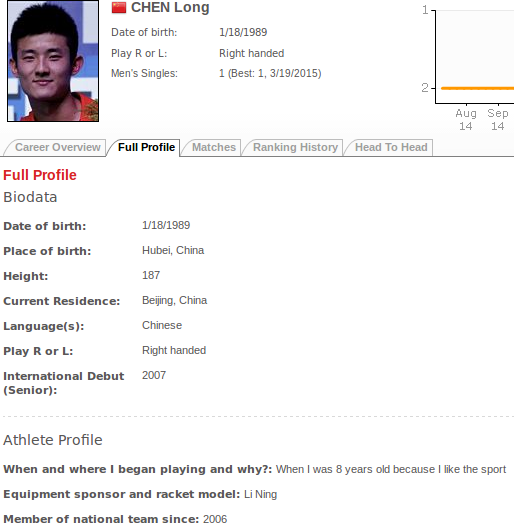
\includegraphics[scale=0.4]{images/bwf_profile}
\caption{Ausschnitt aus der Profilseite der BWF-Webseite}
\label{fig:bwf_profile}
\end{figure}

\section{Gestaltung des Frontends}
Für die Gestaltung des Frontends haben wir uns folgende, mögliche Strukturierung überlegt:\\

\noindent\textbf{Search-Seite mit einer Liste aller Spieler:}
\begin{itemize}
\item Die Seite soll aus zwei Teilen bestehen. Der obere Teil dient zur Spezifizierung von Suchkriterien, während der untere Teil die Ergebnismenge in Form einer Tabelle darstellen soll.
\item Die Filter- und Suchfunktion des oberen Teils der Seite wird mit einem Formular realisiert, in dem zu allen Attributen einer Person Werte spezifiziert werden können. Neben der exakten Suche sollen die Felder auch ähnliche Werte finden (z.B. Eingabe des Nachnamens "`Berg"' liefert Treffer mit Nachnamen "`Berg"' und "`Bergmann"'). Die Eingabefelder sollen den Datentypen der Attribute entsprechend angepasst sein, durch zum Beispiel Textfelder, Auswahllisten, usw.
\item Paging (Auswahlmöglichkeit wie viele Spieler pro Seite angezeigt werden sollen)
\item Das Suchergebnis soll nach Spalten sortierbar sein, sowohl auf-, als auch absteigend.
\item Optional: Benutzer kann die anzuzeigenden Tabellenspalten selber wählen.
\end{itemize}

\noindent\textbf{Detail-Seite für ausgewählten Spieler:}
\begin{itemize}
\item Darstellung aller Informationen zu einem Spieler
\item Anzeige des Profilbildes
\item Attributwerte, die sich aus externen Tabellen ergeben (z.B. club oder nationality) sollen als Hyperlink auf die Search-Seite angezeigt werden, wo alle Spieler mit dem jeweiligen Attribut aufgelistet werden.
\item Wenn Attributwerte nicht gesetzt sind, sollen diese noch nachträglich eintragbar sein. Dazu muss es einen Verweis von dieser Seite auf eine Edit-Seite geben.
\item Optional: Grafik zum Rankingverlauf
\end{itemize}

\noindent\textbf{Profilbearbeitung:}
\begin{itemize}
\item Die Seite sollte nur durch einen Redirect von einer Detail-Seite eines Spielers erreichbar sein.
\item In einem Formular sollen alle Attribute eines Spielers angezeigt werden, die noch nicht gesetzt sind.
\item Nach einem Submit werden die Werte in der Datenbank nachgetragen und man wird zurück zur Detail-Seite verwiesen.
\end{itemize}

\noindent\textbf{Query-Seite zum Erstellen von Abfragen:}
\begin{itemize}
\item Auf dieser Seite wird es ein Freitextfeld geben, wo der Nutzer eigene SQL-Anfragen eintragen kann.
\item Es dürfen nur SELECT-Anfragen ausgeführt werden.
\item Das Ergebnis der Anfrage wird unter dem Freitextfeld in Form einer Tabelle angezeigt.
\end{itemize}

\noindent\textbf{Seite für die grafische Darstellung}
\begin{itemize}
\item Fokussierung auf Häufigkeitsanalysen, da die benutzer-spezifischen Auswertungen zu komplex werden könnten und den Rahmen des Projekts sprengen würden.
\item Darstellungsart der Ergebnisse sollte der Problematik angepasst sein. (Histogramm, Kuchendiagramm, Balkendiagramm) 
\end{itemize}